\chapter{DISCOVERY, LIMITS, MEASUREMENT, AND SENSITIVITY} \label{coinflip}

This chapter briefly covers the statistical methods needed for the $H\rightarrow\mu^+\mu^-$ search. The test of a coin for bias is used as a simple example to explain the concepts of discovery, limits, measurement and sensitivity. These concepts are then extended to a binned counting experiment typical in particle physics. The chapter starts with discovery. 

\section{Discovery}

Many scientific endeavors attempt to disprove some null hypothesis in order to claim the observation of a new effect. For example, to test whether a coin is biased, the experimenter assumes the null hypothesis that the coin is unbiased and then performs an experiment, tossing the coin many times. If all of the tosses are heads, then it's very unlikely that the coin is unbiased, and it's therefore reasonable to rule out the null and to declare the discovery of a biased coin. 

In order to quantify how rarely an unbiased coin would yield an experiment with $N_{heads}$, a model for the probability density function (PDF) is needed. The binomial distribution with $x = N_{heads}$, $\rho = p_{heads} = 0.5$, and $N = N_{tosses}$, is the appropriate PDF,
\begin{equation}
p(x,N;\rho) = \frac{N!}{x! (N - x)!}\rho^{x}(1-\rho)^{N-x}.
\end{equation}
With the PDF, the probability for the null to produce different experiments can be compared in terms of p-values. The p-value assuming the null, $P(x \succ Y|null)$, is the probability to observe something at least as extreme, $\succ$, as the outcome Y given the null. Declaring the cutoff p-value for the coin flipping experiment sets the minimum threshold of heads, $h_{cutoff}$, needed for discovery. Any observation of $x=N_{heads}$ with a p-value rarer than the cutoff, i.e. $P(x \geq h_{cutoff}|null) < p_{cutoff}$, will rule out the null hypothesis. 

Traditionally, different fields require different p-values, and in high energy physics 3$\sigma$ leads to an "observation" and 5$\sigma$ leads to a "discovery". These correspond to p-values of 0.3\% and 0.00006\% respectively. 
\begin{figure}[h!]
  \centering
  \includegraphics[width=3in]{images/stat/p-value.png}
  \caption[An illustrated example of a p-value.]
   {The shaded region represents the p-value for an observation of $N_{heads}=h$. If the p-value for h is lower than the cutoff threshold, then the null hypothesis can be ruled out and a discovery may be declared.}
\label{fig:pvalue_ex}
\end{figure}
As an example, observing 65 heads or greater in 100 tosses occurs just less than 0.3\% of the time for an unbiased coin. Therefore, any experiment with $N_{heads} \geq 65$ would invalidate the null at $3\sigma$ and lead to an observation.

\section{Limits}

Besides discovery, setting a limit is also important. Upon tossing a coin 100 times and finding $N_{heads}=40$, the experimenter may ask which values of $p_{heads}$ are too high to yield such a low observation. In this case, all values of $p_{heads}$ that predict experiments with 40 heads or fewer at too rare a probability may be ruled out at some confidence. For 95\% confidence, $p_{heads} \geq 0.488$ may be ruled out as $p_{heads} \geq 0.488$ yields 40 heads or fewer less than $5\%$ of the time, while smaller values for $p_{heads}$ do not. Therefore, observing 40 heads in 100 tosses places an upper limit of $p_{heads}=0.488$ on the bias of the coin at 95\% confidence. 

\section{Measurement and Uncertainty}
\label{meas}
 
Finally, measuring values is also important. In the case of the coin, the experimenter flips the coin 100 times and attempts to measure how biased the coin is. The value stated as the measured value is usually the best fit, and the best fit value is the one that maximizes the (log) likelihood of seeing the data observed. In practice, minimizing the \textit{negative log likelihood} ($N_{LL}$) is more convenient, 
\begin{equation}
-\frac{\partial}{\partial \rho}ln\left(p(x,N;\rho)\right) = 0 \rightarrow \hat{\rho} = \frac{x}{N}.
\end{equation}   
When performing many independent experiments the PDFs for each experiment multiply and the negative log likelihood is,
\begin{equation}
-ln(p) = -ln\left(\prod_i p_i\right) = -\sum_i ln\left(p_i\right).
\end{equation}
Over many coin flipping experiments, the best fit value for $\rho$ is
\begin{equation}
-\frac{\partial}{\partial \rho}ln(p) = 0 \rightarrow \hat{\rho} = \frac{\sum_{i=1}^{n} x_i}{\sum_{i=1}^{n} N_i}.
\end{equation}
When $N_i$ is the same in each experiment the best fit is just the mean over all experiments,
\begin{equation}
\hat{\rho} = \frac{1}{n} \sum_{i=1}^{n} \frac{x_i}{N} = \frac{1}{n} \sum_{i=1}^{n} \hat{\rho}_i.
\end{equation}
Note that the different experiments all contribute to determine the best fit, and that the results of other experiments constrain the influence of a particular experiment to declare the best fit value.  

In order to quantify the uncertainty of the measured value, limiting values of $\rho$ are computed. The upper limit $\rho_{hi}$ and the lower limit $\rho_{lo}$ define the confidence interval $[\rho_{lo}, \rho_{hi}]$, which quantifies the uncertainty on $\hat{\rho}$. Conceptually, the interval is a range of values for which the observed data (summarized by $\hat{\rho}$) is not too extreme. The confidence interval stated usually corresponds to $1\sigma$ or 68\%, constructed from upper and lower limits that exclude 16\% of their respective PDFs. The construction is illustrated in Figure \ref{fig:meas_uncertainty}, and the construction guarantees that in many experiments the true value will be contained in the confidence interval 68\% of the time.    

\begin{figure}[h!]
  \centering
  \includegraphics[width=6in]{images/stat/plow_and_phi.png}
  \caption[Defining the confidence interval.]
   {The $1\sigma$ uncertainty on $\hat{\rho}$ is determined by finding the appropriate $\rho_{lo}$ and $\rho_{hi}$. $\rho_{lo}$ is the value of $\rho$ just low enough that an observation corresponding to $\hat{\rho}$ or greater occurs only 16\% of the time. $\rho_{hi}$ is the value of $\rho$ just high enough that an observation of $\hat{\rho}$ or less occurs only 16\% of the time. The shaded region represents 16\% of the respective PDF.}
\label{fig:meas_uncertainty}
\end{figure}

Observing 50 heads in 100 tosses leads to $\hat{\rho} = 0.5$ and a corresponding $1\sigma$ confidence interval of $[0.44, 0.56]$. The measurement is then reported as $\hat{\rho} = 0.5^{+0.6}_{-0.6}$. An experiment with more data generally has a lower uncertainty on the measured value. For example, observing 450 heads in 900 tosses leads to $\hat{\rho} = 0.5^{+0.2}_{-0.2}$. Note that the uncertainty shrinks with $\sqrt{N_{tosses}}$, $\frac{0.6}{0.2} = 3 = \sqrt{\frac{900}{100}}$.

\section{Sensitivity}

An analysis is often designed to maximize the chance of discovery by minimizing the expected p-value. The lower the expected p-value given the null, the higher the sensitivity. This section uses a limiting case of the binomial distribution to point out the factors that contribute to a sensitive analysis. Consider an experiment flipping a coin N times, 
\begin{equation}
p(x,N;\rho) = \frac{N!}{x! (N - x)!}\rho^{x}(1-\rho)^{N-x}.
\end{equation}
The experimenter may ask what p-value is expected if the coin has a true value $\rho=\rho_i$. For a coin with $\rho_i$, the observed $N_{heads}$ is most frequently $N\rho_i$. Therefore, given the null with $\rho=\rho_{null}$ one expects
\begin{equation}
p(x=N\rho_i,N;\rho=\rho_{null}) = \frac{N!}{(N\rho_i)! (N - N\rho_i)!}\rho_{null}^{N\rho_i}(1-\rho_{null})^{N-\rho_i}.
\end{equation}
When $N\rho$ is far enough from zero, the binomial distribution may be approximated by a Gaussian with mean $\mu=N\rho$, and standard deviation $\sigma=\sqrt{N\rho(1-\rho)}$. In this limit, the relationship between the expected p-value and the hypotheses are easy to see, because the p-values for a Gaussian are determined by the number of standard deviations away from the mean, Z. The sensitivity is given by $Z=\frac{(x-\mu)}{\sigma}$, and for a coin with $\rho_i$, the expected sensitivity is 
\begin{equation}
Z = \frac{(x-\mu)}{\sigma} = \frac{N(\rho_i - \rho_{null})}{\sqrt{N\rho_{null}(1-\rho_{null})}} = \frac{\sqrt{N}(\rho_i - \rho_{null})}{\sqrt{\rho_{null}(1-\rho_{null})}}.
\end{equation}
The larger Z is, the smaller the p-value, and the more sensitive the experiment. Note that the sensitivity scales as the $\sqrt{N}$, which shows that collecting more data improves the sensitivity to discovery. 

\section{Constraints And Nuisance Parameters}
\label{constraints}

As alluded to in section \ref{meas}, additional measurements provide constraints on the parameters of a PDF. Consider two experiments tossing the same coin with y heads observed in the first experiment and x in the second. In this case, the likelihoods of the individual experiments are multiplied to determine the net likelihood, 
\begin{equation}
p(x, y; \rho) = p(x; \rho)p(y; \rho),
\end{equation}
Upon minimizing the negative log-likelihood, the observations of the first experiment fight with the second experiment to determine the best fit for $\rho$. 

Sometimes it is convenient to replace the actual likelihood of the previous experiment with a suitable representative. Often, a Gaussian is used along with the best fit and the uncertainty of the previous experiment, $\hat{\rho}_{y}$ and $\sigma_y$. The net likelihood then becomes,
\begin{equation}
p(x; \rho) = p(x; \rho) \mathcal{N}(\hat{\rho}_y; \mu=\rho, \sigma=\sigma_y).
\end{equation}
The Gaussian ($\mathcal{N}$) fights to keep $\hat{\rho}$ near $\hat{\rho}_y$ with a strength dependent on $\sigma_y$. Other constraints like the log-normal or Poisson distributions are also used. Constraint terms are especially useful when they replace a complicated likelihood with many data points. 

Imagine a case where the distribution of dirt on a coin affects the net bias $\rho$. The fraction of heads expected then depends on the bias of the coin itself and the additional bias from the dirt, $\rho = \rho_{coin} + \rho_{dirt}$. If a complicated measurement is made to determine the distribution of dirt on the coin, thus estimating $\rho_{dirt}$, then the bias of the coin itself $\rho_{coin}$ can be extracted. The net likelihood includes the likelihood for the set of observations y
\begin{equation}
p(x, y; \rho_{coin}, \rho_{dirt}) = p(x; \rho_{coin}, \rho_{dirt})p(y; \rho_{dirt}).
\end{equation}

The observations y determine the best fit $\hat{\rho}_{y-dirt}$ and uncertainty $\sigma_{y-dirt}$ from that experiment, and the likelihood becomes, 
\begin{equation}
p(x, \hat{\rho}_{y-dirt}; \rho_{coin}, \rho_{dirt}) = p(x; \rho_{coin}, \rho_{dirt})
                                   \mathcal{N}(\hat{\rho}_{y-dirt}; \mu=\rho_{dirt}, \sigma=\sigma_{y-dirt}),
\end{equation}
where a Gaussian constraint replaces the complicated likelihood of the $\rho_{dirt}$ measurement involving the data points y. The best fit for $\rho_{coin}$ can be calculated using the maximum likelihood estimates for $\rho_{coin}$ and $\rho_{dirt}$ given x and $\hat{\rho}_{y-dirt}$. Limits and uncertainty on $\rho_{coin}$ can be calculated by \textit{profiling} the likelihood,  
\begin{equation}
p(x, \hat{\rho}_{y-dirt}; \rho_{coin}, \hat{\hat{\rho}}_{dirt}) = p(x; \rho_{coin}, \hat{\hat{\rho}}_{dirt})
                                   \mathcal{N}(\hat{\rho}_{y-dirt}; \mu=\hat{\hat{\rho}}_{dirt}, \sigma=\sigma_{y-dirt}).
\end{equation}
The double hat designates a maximum likelihood estimate of the parameter for fixed $\rho_{coin}$. The parameters other than the parameter of interest are called \textit{nuisance parameters}, and profiling sets the nuisance parameters to their best fit estimates for some fixed value of the parameter of interest. 

The distribution for $p(x, \hat{\rho}_{y-dirt}; \rho_{coin}, \hat{\hat{\rho}}_{dirt})$ can be simulated using Monte Carlo methods, where $\hat{\rho}_{y-dirt}$ is a random variable drawn from $\mathcal{N}(\hat{\rho}_{y-dirt}; \mu=\hat{\hat{\rho}}_{dirt}, \sigma=\sigma_{y-dirt})$. The randomness of $\hat{\rho}_{y-dirt}$ smears the distribution for $\hat{\rho}_{coin}$ and widens its uncertainty. The uncertainty of $\hat{\rho}_{y-dirt}$ also leads to looser the limits on $\rho_{coin}$.

\section{A Particle Physics Search}

This section extends the previous concepts to the search for a new particle in high energy particle physics. Such a search makes use of two hypotheses: the background only (B) and the signal plus background (S+B). The background only predicts the number of events if the particle does not exist, and the signal plus background (S+B) predicts the number of events if the particle does exist. The signal (S) represents the number of additional events expected if the new particle exists.

\begin{figure}[h!]
  \centering
  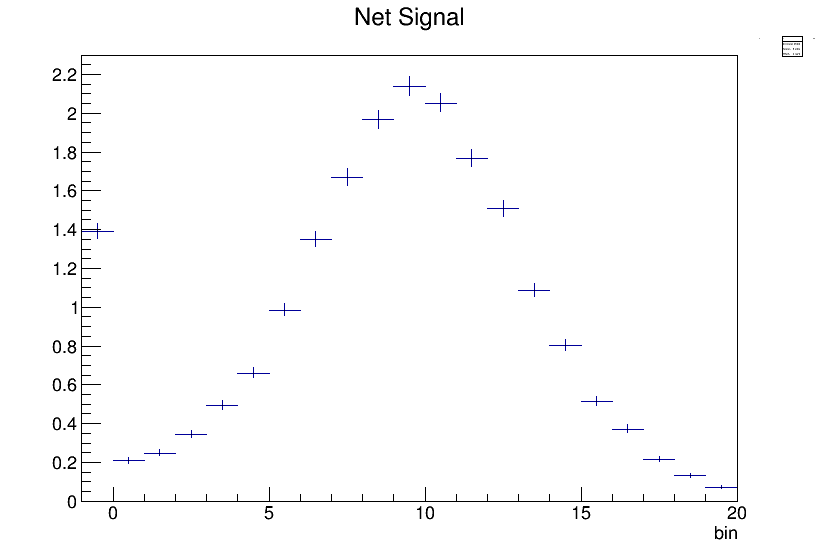
\includegraphics[width=0.49\linewidth]{images/bdt_cats/binning_signal_example.png}
  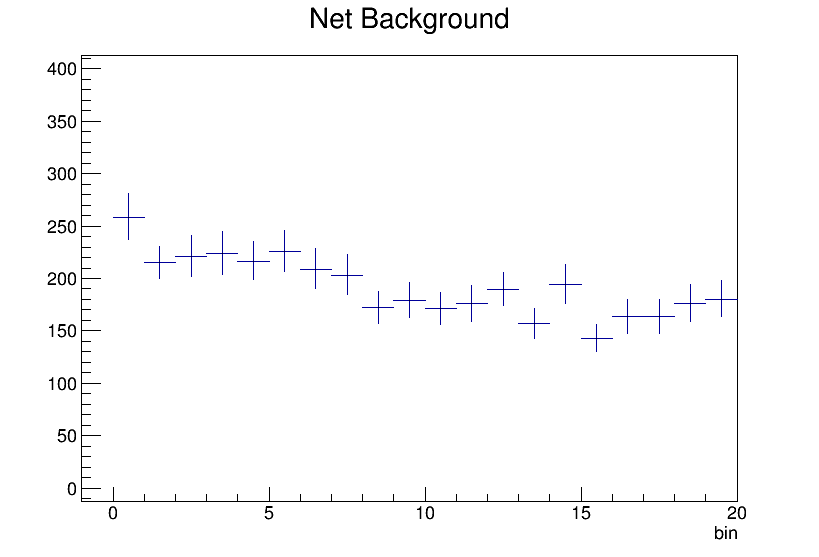
\includegraphics[width=0.49\linewidth]{images/bdt_cats/binning_bg_example.png}
  \caption[An example of the signal and background used for the background only and S+B hypotheses.]
  {An example of the binned signal and background used for the background only and S+B hypotheses.}
  \label{fig:sb_binning_example}
\end{figure}

The S+B and B hypotheses are usually one dimensional distributions binned along some variable. If the observed distribution of events is too different from the background only, the background only hypothesis is ruled out and the experiment proclaims the discovery of a new particle. The distribution describing the amount of signal (S) is often reported in terms of the signal strength ($\nu$) \footnote{Usually $\mu$ denotes the signal strength, but $\mu$ was already used in this section to designate the Gaussian mean.} and the SM prediction (s) allowing the signal hypothesis to be written $S = \nu s$. A signal strength of 1 means that the signal model S is simply the Standard Model prediction, and a signal strength of 2 means that S has twice the signal as the SM prediction in each bin.  

The probability to observe a particular count in a bin is described by the Poisson distribution
\begin{equation}
p\left( x; \lambda \right) = \frac{{e^{ - \lambda } \lambda^x }}{{x!}},
\end{equation}
where $\lambda$ is the expected number of events and x is the observed number of events. A valid hypothesis provides the expected number of events in each bin and the data provides the observed number in each bin. The expected number of events in a bin is given by $\lambda$ and the standard deviation is $\sigma = \sqrt{\lambda}$. When $\lambda$ is far enough from zero the Poisson distribution may be described by a Gaussian with mean $\mu = \lambda$ and standard deviation $\sigma = \sqrt{\lambda}$.  

\subsection{Sensitivity}
\label{sensitivity}

The sensitivity becomes much more interesting with binned distributions. First consider the sensitivity for a single bin. If the Standard Model or some other theory predicts the expected number of events in a bin to be $\lambda_i=S_i+B_i$ and the null predicts $\lambda_i=B_i$, then the expected sensitivity for discovery is,
\begin{equation}
Z = \frac{(x_i-\mu_i)}{\sigma_i} = \frac{(S_i+B_i-B_i)}{\sqrt{B_i}} = \frac{S_i}{\sqrt{B_i}} = \frac{\sqrt{N}\rho_{si}}{\sqrt{\rho_{bi}}}.
\end{equation}
As before, this scales with the $\sqrt{N}$. So, again, one way to ensure a sensitive experiment is to collect a lot of data, but that's not the only way. With many bins, the PDFs for each bin multiply and the $N_{LL}$ in the Gaussian limit is,
\begin{equation}
\label{eq:norm}
-ln\left(\frac{p}{C}\right) = -ln\left(\prod_i p_i\right) + ln\left( C \right) 
                            = -\sum_i ln\left(p_i\right) + ln\left( C \right) 
                            = \sum_i \frac{(x_i-\mu_i)^2}{2\sigma_i^2},
\end{equation}
where C is the sum of the normalizations for the Gaussians. After normalizing by C and the factor of 2, the $N_{LL}$ is a sum of $\chi^2$ variables and therefore itself a $\chi^2$ variable, 
\begin{equation}
\chi^2_{nll} = -2ln\left(\frac{p}{C}\right) = \sum \frac{(x_i-\mu_i)^2}{\sigma_i^2}.
\end{equation}
This shows that the expected sensitivity with many Poissonian bins may be estimated by
\begin{equation}
Z^2 = \frac{(x_{nll}-\mu_{nll})^2}{\sigma_{nll}^2} = \sum_i \frac{S_i^2}{B_i}.  
\end{equation}
By concentrating the fixed amount of signal into a few bins with low background the sensitivity may improve regardless of the data available. This is indicative of the idea that the null may be invalidated when the data observed is many times the expected fluctuations.

\subsection{Test Statistic}

The negative log likelihood can be used to form the test statistic t, a random variable that summarizes the total discrepancy between the observed data and a given theory. The statistic is nice because it reduces the multitude of discrepancies in the many bins to a single number. The test statistic t is given by, 
\begin{equation}
t = -2ln\left(\frac{p(x_i,\theta)}{p(x_i,\hat{\theta})}\right).
\end{equation}
The normalization, $p(x_i,\hat{\theta})$, is the PDF with the parameters set to the best fit values, and this term as in Equation \ref{eq:norm} sets the range of t from zero to infinity. When there is only one parameter of interest $\nu$ the likelihood may be reduced to one dimension by profiling the nuisance parameters $\theta$,
\begin{equation}
t = -2ln\left(\frac{p(x_i,\nu,\hat{\hat{\theta}})}{p(x_i,\hat{\theta})}\right).
\end{equation}
As before, the $\hat{\hat{\theta}}$ parameters are the best fit values for a fixed parameter of interest $\nu$. The profiled test statistic may be used to set limits on the parameter of interest. Asymptotically, the test statistic is a $\chi^2$ variable. See the analysis of section \ref{sensitivity}. Constraints may be included as necessary. 

\subsection{Constraints}

When previous fits have been performed to determine certain parameters and their uncertainty, the likelihoods can be included to encode the information. The measurements on the nuisance parameters $\theta$ are included like so,
\begin{equation}
p(x_i; \nu, \theta) = \prod_i Poisson(x_i, \lambda_i(\nu, \theta))\prod_j p(y_j, \theta_j),
\end{equation}
where $y_j$ represents the previously observed data and $\nu$ represents the signal strength. As in section \ref{constraints}, the observations $y_j$ are summarized by the best fits ($\bar{\theta_j}$) rather than keeping track of the actual data. The net likelihood becomes,
\begin{equation}
p(x_i; \nu, \theta) = \prod_i Poisson(x_i; \lambda_i(\nu, \theta))\prod_j C(\bar{\theta_j}, \theta_j, \sigma_j),
\end{equation}
where C designates some constraint PDF. Constraints implement the various systematic and theoretical uncertainties involved in the analysis.  

\section{Using The Test Statistic}

With a model for the expected yields in each bin, the distribution for t may be approximated by Monte Carlo methods, or by assuming that with enough data t reduces to a $\chi^2$ distribution. The expected p-value against the background only may be calculated using the expected yields for S+B as the expected hypothesis and the background only yields as the null. Similarly, the expected upper limit on S may be calculated using t with S+B as the null and the background as the expected hypothesis. The expected upper limit at 95\% confidence is calculated by finding the value of S high enough that observing the expected background-only has a p-value of 5\%. A higher expected sensitivity and lower expected upper limit are important goals in the design of a physics analysis.

Upon collecting data, the test statistic t may be used with the data observed and the background only as the null to check for discovery. The observed upper limit on S at 95\% confidence is computed by finding a high enough value of S such that observing the data has a p-value of $5\%$. These can be compared to the expected p-value and the expected upper limit. 
 
In high energy physics the CLs method is often used to set the upper limits. The CLs method reports an upper limit using an adjusted p-value, $p_{CLs} = \frac{p_\mu}{p_{bkg-only}}$, where $p_{\mu}$ is the probability for a theory with a true parameter $\mu$ to observe x or less data and $p_{bkg-only}$ is the probability for the background only to observe x or less data. Using the CLs method at 95\% confidence, $p_\mu$ must be $0.05p_{bkg-only}$ or less. When the data observed is much greater than the median expected background, the integrated probability less than the observed is most of the distribution, $p_{bkg-only}$ goes to 1, and the CLs upper limit approaches the standard upper limit. But in general, $p_{bkg-only}$ is less than one yielding a $p_{CLs}$ greater than $p_\mu$ and a CLs limit that is more conservative than the standard upper limit. The CLs construction guarantees that hypotheses with low $p_{\mu}$ must also differ substantially from the background to be ruled out.   


%%%%%%%%%%%%%%%%%%%%%%%%%%%%%%% SOME SAVED INFO ON LIMITING CASE FOR UNCERTAINTY %%%%%%%%%%%%%%%%%%%%%%%%

%When the likelihood is Gaussian the interval is simply $\hat{\mu} \pm \sigma$. In the limit of large statistics, the likelihood becomes Gaussian, and the negative log-likelihood, simplifies to
%\begin{equation}
%N_{LL} = -ln[p] = -ln\left[Ae^{\frac{(x-\mu)^2}{2\sigma^2}}\right]= -ln[A] + \frac{(x-\mu)^2}{2\sigma^2}.
%\end{equation}
%Expanding about the minimum, $\hat{\mu}$, provides an estimate of $\sigma$ and hence the confidence interval, 
%\begin{equation}
%N_{LL}(\hat{\mu}) + 0(x-\hat{\mu}) + \frac{1}{2}N_{LL}''(\hat{\mu})(x-\hat{\mu})^2 = -ln[A] + \frac{(x-\hat{\mu})^2}{2\sigma^2} \rightarrow \sigma^2 = \frac{1}{N_{LL}''(\hat{\mu})}.
%\end{equation}
%Note that $\sigma$ may be determined by moving x away from the minimum until $\Delta N_{LL} = 1$. The $\Delta N_{LL} = 1$ method is sometimes used as an estimate of the uncertainty even when the likelihood is not Gaussian. In some cases the PDF may be multidimensional, and in those cases, $\sigma^2$ is the covariance matrix with $\partial_{\theta_i}\partial_{\theta_j}N_{LL}(\hat{\theta}) = (\sigma^2)^{-1}_{ij}$. Multidimensional or otherwise, $\sigma$ can be used to estimate the uncertainty on the best fit values. 
